\documentclass[11pt,a4paper]{article}
\usepackage[latin1]{inputenc}
\usepackage{amsmath}
\usepackage{amsfonts}
\usepackage{amssymb}
\usepackage{array}
\usepackage{graphicx}
\author{Jordan Murray}
\title{EECS305 Lab5}
\begin{document}
\begin{center}
\fontsize{24}{12}\selectfont
\textbf{Experiment 6: State Feedback Control of a DC Servo Motor System}
\end{center}

\section{OBJECTIVES}
\begin{itemize}
\item To demonstrate how properties of a closed-loop system are influenced by the closed-loop roots.
\item To introduce pole placement by state feedback design for a continuous system.
\item To obtain the state space model for DC servo system.
\end{itemize}

\section{BASIC KNOWLEDGE}
In this section we introduce mathematical models in state space for a DC servomechanism.

A block diagram for a typical servomechanism is shown in Fig. ~\ref{fig:servostatespaceblock}. The action of the servomechanism is to track a desired position (speed) despite the presence of disturbance inputs to the process.

\begin{figure}[here]
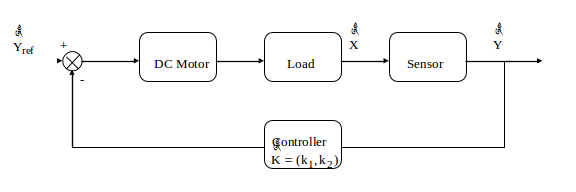
\includegraphics[width=\textwidth]{imglab/servostatespaceblock.png}
\caption{Servomechanism block diagram}
\label{fig:servostatespaceblock}
\end{figure}

\subsection{Model Development}

\begin{figure}[here]
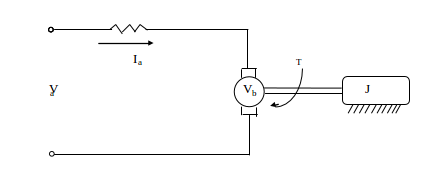
\includegraphics[width=\textwidth]{imglab/servoschemdiagram.png}
\caption{schematic diagram of the DC servo motor}
\label{fig:servoschem}
\end{figure}

We begin by developing a simplified linear model of an armature controlled DC-Servo motor and load. Fig. ~\ref{fig:servoschem} shows the schematic diagram of the motor and load.

Neglecting the inductance of the armature circuit, the armature voltage $V_{a}$ produces a current $I_{a}$ as given by:

\begin{equation} \label{eq:1}
I_{a} = \frac{V_{a}-V_{b}}{R_{a}}
\end{equation}

Here $V_{b}$ denotes the back emf of the motor and $R_{a}$ is the armature resistance.

\begin{equation} \label{eq:2}
T=K_{T}I_{a}
\end{equation}

But from Newton's law, assuming an inertia load and neglecting load damping:

\begin{equation} \label{eq:3}
T = J\ddot{\theta}
\end{equation}

combining equations \ref{eq:1}, \ref{eq:2}, and \ref{eq:3} we obtain:

\begin{equation} \label{eq:4}
K_{T}\left[\frac{V_{a}-V_{b}}{R_{a}}\right] = J\ddot{\theta}
\end{equation} 

Using the relationship V$_{b}$ = K$_{b}\dot{\theta}$ and, letting V$_{a}$ = U (input signal), we have:

\begin{equation} \label{eq:5}
\frac{K_{T}}{R_{a}}\left[U-K_{b}\dot{\theta}\right] = J\ddot{\theta}
\end{equation}

\begin{equation} \label{eq:6}
\frac{JR_{a}}{K_{T}}\ddot{\theta}+ K_{b}\dot{\theta} = U
\end{equation}

\begin{equation} \label{eq:7}
\ddot{\theta} + \frac{K_{b}K_{T}}{JR_{a}}\dot{\theta} = \frac{K_{T}}{JR_{a}}U
\end{equation}

Equation ~\ref{eq:7} is the differential equation for the DC motor.

Let $\frac{K_{b}K_{T}}{JR_{a}}=\frac{1}{T_{s}}$, $\frac{K_{T}}{JR_{a}} = \frac{K_{0s}}{s(T_{s}s+1)}$. Here $K_{0s}$ is the static gain and $T_{s}$ is the time constant of the system from input voltage to output speed. From D.E.~\ref{eq:7} we can have the following transfer function:

\begin{equation} \label{eq:8}
\frac{\theta(s)}{U(s)} = \frac{K_{0s}}{s(T_{s} s + 1)}
\end{equation}

Considering the measurements of speed and position, the system can be depicted as in Fig. ~\ref{fig:servomeasschem}:

\begin{figure}[here]
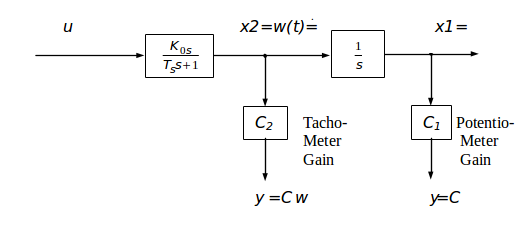
\includegraphics[width=\textwidth]{imglab/servomeasurementschematic.png}
\caption{schematic of the DC motor system with measurements}
\label{fig:servomeasschem}
\end{figure}

Then, the second order D.E. of the DC-motor can be rewritten in state-space format:

\begin{equation} \label{eq:9}
\dot{x} = Ax  + Bu 
 y = Cx
\end{equation}

where, $x = \left[\begin{matrix}x_{1} \\ x_{2}\end{matrix}\right]$, $u=u$, $y = \left[\begin{matrix}y_{1} \\ y_{2}\end{matrix}\right]$, and
$A = \left[\begin{matrix}0 & 1 \\ 0 & -\frac{1}{\tau}\end{matrix}\right]$, $B=\left[\begin{matrix} 0 \\ \frac{K_{s}}{\tau} \end{matrix}\right]$, $C = \left[\begin{matrix}C_{1} & 0 \\ 0 & C_{2} \end{matrix}\right]$

\subsection{State space design method} \label{method}
Using a state feedback controller, we want to to position the closed-loop poles of of the system. There are different ways of achieving this. One of the design methods is described below.

The continuous-time system is represented by the state equation:

$\dot{x} = Ax + Bu$
$y = Cx$

A,B,C is a 2 by 2 matrix defined as above.

The state controller realizes a linear feedback control law of the form:

\begin{equation}
u = -K(y_{d}-y) = -KC(x_{d} - x)
\end{equation}

Where K = $[k_{1} k_{2}]$ is a feedback gain vector.

We require that the roots of the closed-loop system be equal to $\lambda_{1}$, $\lambda_{2}$. The design method consists of finding a K such that the roots of the closed-loop system are in the desired locations. It can be shown that there exists a linear feedback law that gives a closed-loop system with roots specified only if the pair (A,B) is controllable.

Define $C_{s}=C_{1}/C_{2}$ and $K_{s}=C_{2}K_{0s}$, then the state matrix of the closed-loop system is:
$A_{c} = A-BKC = \left[\begin{matrix} 0 & 1 \\ 0 & -\frac{1}{T_{s}} \end{matrix}\right]-\left[\begin{matrix} 0 \\  -\frac{K_{0s}}{T_{s}} \end{matrix}\right]\left[\begin{matrix} k_{1} & k_{2} \end{matrix}\right]\left[\begin{matrix} C_{1} & 0 \\ 0 & C_{2} \end{matrix}\right] = \left[\begin{matrix} 0 & 1 \\ -\frac{k_{1}C_{s}K_{0s}}{T_{s}} & -\frac{1+k_{2}C_{2}K_{0s}}{T_{s}} \end{matrix} \right] = \left[\begin{matrix} 0 & 1 \\ -\frac{k_{1}\frac{C_{1}}{C_{2}}C_{2}K_{0s}}{T_{s}} & -\frac{1+k_{2}C_{2}K_{0s}}{T_{s}} \end{matrix} \right] = \left[\begin{matrix} 0 & 1 \\ -\frac{k_{1}C_{s}K_{s}}{T_{s}} & -\frac{1+k_{2}K_{s}}{T_{s}} \end{matrix} \right]$

and the characteristic equation is:

\begin{equation}
C(s) = \mathrm{det}(\lambda I - A_{c}) = \lambda^{2} + \lambda \frac{1 + K_{s}k_{2}}{T_{s}}+\frac{K_{s}k_{1}C_{s}}{T_{s}} = 0
\end{equation}

By means of the feedback gains, the roots of the characteristic equation may be changed. From Vieta's formula we obtain:

\begin{equation}
\lambda_{1}\cdot\lambda_{2} = \frac{K_{s}C_{s}k_{1}}{T_{s}}    \qquad   \lambda_{1} + \lambda_{2} = -\frac{1+K_{s}k_{2}}{T_{s}}
\end{equation}

and we can calculate $k_{1}$ and $k_{2}$ from:

\begin{equation}
k_{1} = \frac{\lambda_{1}\lambda_{2}T_{s}}{K_{s}C_{s}} \qquad k_{2} = -\frac{(\lambda+\lambda_{2})T_{s}+1}{K_{s}}
\end{equation}

Then you can use the parameters ($K_{s}$,$T_{s}$,$C_{s}$) that you determined for the servo motor in Lab 5 to design the feedback gains.

\section{EXPERIMENTAL PROCEDURES}
We will be designing state controllers to position the closed-loop poles of the DC servo system in several different places.

\begin{enumerate}
\item Open Matlab and open the Simulink model \textbf{Lab6\_StateFB.slx}.
\item Design a controller according to the procedure of section \ref{method} to position the roots as follows: $\lambda_{1}=-2, \lambda_{2}=-4$. Enter the values for $k_{1}$ and $k_{2}$ in the gain blocks.
\item Run the simulation
\item Find the scope data in the workspace and save it to a .mat file using the save command.
\item Repeat the above for the following pairs of root locations:
\begin{enumerate}
\item $\lambda_{1}=-4, \lambda_{2}=-5$
\item $\lambda_{1,2} = -2 \pm 2j$
\item $\lambda_{1,2} = -2 \pm 4\sqrt{6}j$
\end{enumerate}

\end{enumerate}

\section{EXERCISES}
\begin{enumerate}
\item Fill in the following table:
\begin{center}
\begin{tabular}{| >{\centering}p{3cm} | >{\centering}p{.75cm} | >{\centering}p{.75cm} | c | c |}
	\hline
	 Poles & $k_{1}$ & $k_{2}$ & $\zeta$ & $\omega_{n}$ \\ \hline
	 & & & N/A & N/A \\ \hline
	 & & & N/A & N/A \\ \hline
	 & & & & \\ \hline
	 & & & & \\ \hline
\end{tabular}
\end{center}

\item Explain the results.
\item Compute the rank of [B AB]. 
\end{enumerate}

\end{document}